\documentclass{beamer}
\usepackage[utf8]{inputenc}
\usepackage{graphicx, epsfig}
\usepackage{amsmath,mathrsfs,amsfonts,amssymb}
\usepackage{floatflt}
\usepackage{epic,ecltree}
\usepackage{mathtext}
\usepackage{fancybox}
\usepackage{fancyhdr}
\usepackage{multirow}
\usepackage{enumerate}
\usepackage{epstopdf}
\usepackage{multicol}
\usepackage{algorithm}
\usepackage[noend]{algorithmic}
\usepackage{tikz}
\usepackage{blindtext}
\usetheme{default}%{Singapore}%{Warsaw}%{Warsaw}%{Darmstadt}
\usecolortheme{default}

\setbeamerfont{title}{size=\Huge}
\setbeamertemplate{footline}[page number]{}

\setbeamertemplate{section in toc}[sections numbered]


\makeatletter
\newcommand\HUGE{\@setfontsize\Huge{35}{40}}
\makeatother    

\setbeamerfont{title}{size=\HUGE}
\beamertemplatenavigationsymbolsempty

% latin bold lower
\newcommand{\ba}{\mathbf{a}} 
\newcommand{\bc}{\mathbf{c}} 
\newcommand{\be}{\mathbf{e}} 
\newcommand{\bff}{\mathbf{f}} % \bf - for bold type
\newcommand{\bg}{\mathbf{g}} 
\newcommand{\bh}{\mathbf{h}} 
\newcommand{\bp}{\mathbf{p}} 
\newcommand{\bq}{\mathbf{q}} 
\newcommand{\bt}{\mathbf{t}} 
\newcommand{\bs}{\mathbf{s}} 
\newcommand{\bu}{\mathbf{u}} 
\newcommand{\bv}{\mathbf{v}} 
\newcommand{\bw}{\mathbf{w}} 
\newcommand{\bx}{\mathbf{x}} 
\newcommand{\by}{\mathbf{y}} 
\newcommand{\bz}{\mathbf{z}} 

% latin bold upper
\newcommand{\bA}{\mathbf{A}} 
\newcommand{\bB}{\mathbf{B}} 
\newcommand{\bC}{\mathbf{C}} 
\newcommand{\bG}{\mathbf{G}} 
\newcommand{\bI}{\mathbf{I}} 
\newcommand{\bJ}{\mathbf{J}} 
\newcommand{\bL}{\mathbf{L}} 
\newcommand{\bM}{\mathbf{M}} 
\newcommand{\bP}{\mathbf{P}}
\newcommand{\bQ}{\mathbf{Q}} 
\newcommand{\bR}{\mathbf{R}} 
\newcommand{\bT}{\mathbf{T}} 
\newcommand{\bU}{\mathbf{U}} 
\newcommand{\bV}{\mathbf{V}} 
\newcommand{\bW}{\mathbf{W}} 
\newcommand{\bX}{\mathbf{X}} 
\newcommand{\bY}{\mathbf{Y}} 
\newcommand{\bZ}{\mathbf{Z}} 

% latin cal upper
\newcommand{\cF}{\mathcal{F}} 
\newcommand{\cG}{\mathcal{G}} 
\newcommand{\cI}{\mathcal{I}} 
\newcommand{\cL}{\mathcal{L}} 
\newcommand{\cM}{\mathcal{M}} 
\newcommand{\cN}{\mathcal{N}} 
\newcommand{\cP}{\mathcal{P}} 
\newcommand{\cS}{\mathcal{S}} 
\newcommand{\cT}{\mathcal{T}} 
\newcommand{\cW}{\mathcal{W}} 
\newcommand{\cX}{\mathcal{X}} 
\newcommand{\cZ}{\mathcal{Z}} 

% latin bb upper
\newcommand{\bbE}{\mathbb{E}} 
\newcommand{\bbI}{\mathbb{I}} 
\newcommand{\bbP}{\mathbb{P}} 
\newcommand{\bbR}{\mathbb{R}} 

% greek bold lower
\newcommand{\bepsilon}{\boldsymbol{\epsilon}} 
\newcommand{\btheta}{\boldsymbol{\theta}} 
\newcommand{\blambda}{\boldsymbol{\lambda}} 
\newcommand{\bpi}{\boldsymbol{\pi}} 
\newcommand{\bmu}{\boldsymbol{\mu}} 
\newcommand{\bsigma}{\boldsymbol{\sigma}} 
\newcommand{\bphi}{\boldsymbol{\phi}} 

% greek bold upper
\newcommand{\bSigma}{\boldsymbol{\Sigma}} 

\DeclareMathOperator*{\argmin}{arg\,min}
\DeclareMathOperator*{\argmax}{arg\,max}

\newcommand{\createdgmtitle}[1]{\title[\hbox to 56mm{Deep Generative Models  \hfill\insertframenumber\,/\,\inserttotalframenumber}]
	{\vspace{1cm} \\ \textbf{Deep Generative Models} \\ {\Huge Lecture #1}}
	\author{Roman Isachenko}
		\institute{
\includegraphics[width=0.7cm]{../utils/aimasterslogo} \LARGE{AI Masters}}
	\date{2024, Spring}
}

\usepackage{tikz}
\usetikzlibrary{arrows,shapes,positioning,shadows,trees}

\newcommand\myfootnote[1]{%
  \tikz[remember picture,overlay]
  \draw (current page.south west) +(1in + \oddsidemargin,0.5em)
  node[anchor=south west,inner sep=0pt]{\parbox{\textwidth}{%
      \rlap{\rule{10em}{0.4pt}}\raggedright\scriptsize \textit{#1}}};}

\newcommand\myfootnotewithlink[2]{%
  \tikz[remember picture,overlay]
  \draw (current page.south west) +(1in + \oddsidemargin,0.5em)
  node[anchor=south west,inner sep=0pt]{\parbox{\textwidth}{%
      \rlap{\rule{10em}{0.4pt}}\raggedright\scriptsize\href{#1}{\textit{#2}}}};}
      
\AtBeginSection[]
      {
      	\begin{frame}{Outline}
      		\tableofcontents[currentsection]
      	\end{frame}
      }
      \AtBeginSubsection[]{
      	\begin{frame}{Outline}
      		\tableofcontents[currentsection,currentsubsection]
      	\end{frame}
}
\createdgmtitle{13}

%--------------------------------------------------------------------------------
\begin{document}
%--------------------------------------------------------------------------------
\begin{frame}[noframenumbering,plain]
%\thispagestyle{empty}
\titlepage
\end{frame}
%=======
\begin{frame}{Recap of previous lecture}
	\vspace{-0.2cm}
	\begin{block}{SDE basics}
		Let define stochastic process $\bx(t)$ with initial condition $\bx(0) \sim p_0(\bx)$:
		\[
			d\bx = \mathbf{f}(\bx, t) dt + g(t) d \bw, 
		\]
		where $\bw(t)$ is the standard Wiener process (Brownian motion)
		\vspace{-0.2cm}
		\[		
			\bw(t) - \bw(s) \sim \cN(0, (t - s) \bI), \quad d \bw = \bepsilon \cdot \sqrt{dt}, \, \text{where } \bepsilon \sim \cN(0, \bI).
		\]
	\end{block}
	\vspace{-0.3cm}
	\begin{block}{Discretization of SDE (Euler method)}
		\vspace{-0.3cm}
		\[
			\bx(t + dt) = \bx(t) + \bff(\bx(t), t) \cdot dt + g(t) \cdot \bepsilon \cdot \sqrt{dt}
		\]
		\vspace{-0.3cm}
	\end{block}
	\begin{itemize}
		\item At each moment $t$ we have the density $p_t(\bx) = p(\bx, t)$.
		\item $p: \bbR^m \times [0, 1] \rightarrow \bbR_+$ is a \textbf{probability path} between $p_0(\bx)$ and $p_1(\bx)$.
	\end{itemize}
\end{frame}
%=======
\begin{frame}{Recap of previous lecture}
 	\begin{block}{Theorem (Kolmogorov-Fokker-Planck)}
 		Evolution of the distribution $p_t(\bx)$ is given by the following equation:
 		\vspace{-0.3cm}
 		\[
 			\frac{\partial p_t(\bx)}{\partial t} = - \text{div}\left(\bff(\bx, t) p_t(\bx)\right) + \frac{1}{2}g^2(t) \Delta_{\bx}p_t(\bx)
 		\]
 		\vspace{-0.5cm}
 	\end{block}
 	\begin{block}{Langevin SDE (special case)}
 		\vspace{-0.3cm}
 		\[
 			d \bx = {\color{violet}\frac{1}{2} \frac{\partial}{\partial \bx} \log p_t(\bx)} d t + {\color{teal} 1 } \cdot d \bw
 		\]
 		\vspace{-0.3cm}
 	\end{block}
 	The density $p(\bx | \btheta)$ is a \textbf{stationary} distribution for the SDE.
	\begin{block}{Langevin dynamics}
		Samples from the following dynamics will comes from $p(\bx | \btheta)$ under mild regularity conditions for small enough $\eta$.
		\vspace{-0.2cm}
		\[
			\bx_{t + 1} = \bx_t + \frac{\eta}{2} \nabla_{\bx_t} \log p(\bx_t | \btheta) + \sqrt{\eta} \cdot \bepsilon, \quad \bepsilon \sim \cN(0, \bI).
		\]
	\end{block}
	\myfootnotewithlink{https://www.stats.ox.ac.uk/~teh/research/compstats/WelTeh2011a.pdf}{Welling M. Bayesian Learning via Stochastic Gradient Langevin Dynamics, 2011}
\end{frame}
%=======
\begin{frame}{Recap of previous lecture}
	\vspace{-0.5cm}
	\[
		d\bx = \mathbf{f}(\bx, t) dt + g(t) d \bw - \text{SDE with the probability path } p_t(\bx)
	\]
	\vspace{-0.5cm}
	\begin{block}{Probability flow ODE}
		There exists ODE with identical the probability path $p_t(\bx)$ of the form
		\[
			d\bx = \left(\mathbf{f}(\bx, t) -\frac{1}{2} g^2(t) \frac{\partial}{\partial \bx} \log p_t(\bx) \right) dt
		\]
		\vspace{-0.3cm}
	\end{block}
	\begin{figure}
		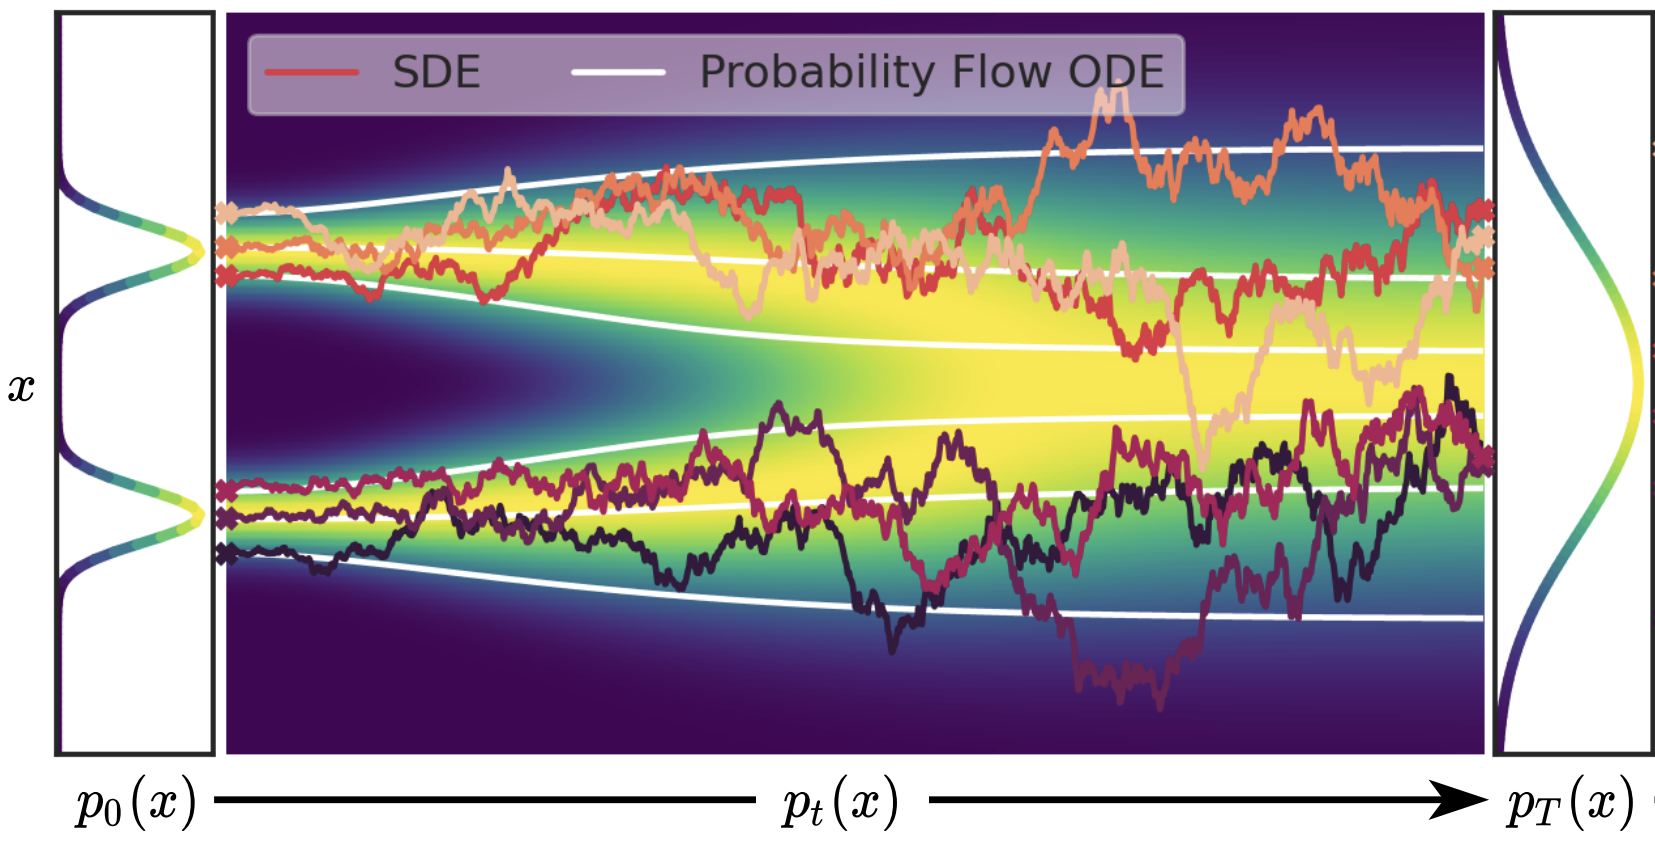
\includegraphics[width=0.75\linewidth]{figs/probability_flow}
	\end{figure}
	\myfootnotewithlink{https://arxiv.org/abs/2011.13456}{Song Y., et al. Score-Based Generative Modeling through Stochastic Differential Equations, 2020}
\end{frame}
%=======
\begin{frame}{Recap of previous lecture}
	\vspace{-0.3cm}
	\[
		d\bx = \mathbf{f}(\bx, t) dt, \quad \bx(t + dt) = \bx(t) + \mathbf{f}(\bx, t) dt
	\]
	\vspace{-0.5cm}
	\begin{block}{Reverse ODE}
		Let $\tau = 1 - t$ ($d\tau = -dt$).
		\vspace{-0.3cm}
		\[
			d\bx = - \bff(\bx, 1 - \tau) d \tau
		\]
	\end{block}
	\vspace{-0.5cm}
	\begin{block}{Reverse SDE}
		There exists the reverse SDE for the SDE $d\bx = \mathbf{f}(\bx, t) dt + g(t) d \bw$ that has the following form
		\vspace{-0.3cm}
		\[
			d\bx = \left(\mathbf{f}(\bx, t) {\color{violet}- g^2(t) \frac{\partial}{\partial \bx}\log p_t(\bx)}\right) dt + g(t) d \bw, \quad dt < 0
		\] 
	\end{block}
	\vspace{-0.5cm}
	\begin{block}{Sketch of the proof}
		\begin{itemize}
			\item Convert initial SDE to probability flow ODE.
			\item Revert probability flow ODE.
			\item Convert reverse probability flow ODE to reverse SDE.
		\end{itemize}
	\end{block}
	\myfootnotewithlink{https://arxiv.org/abs/2011.13456}{Song Y., et al. Score-Based Generative Modeling through Stochastic Differential Equations, 2020}
\end{frame}
%=======
\begin{frame}{Recap of previous lecture}
	\vspace{-0.5cm}
	\begin{align*}
		d\bx &= \mathbf{f}(\bx, t) dt + g(t) d \bw - \text{SDE} \\
		d\bx &= \left(\mathbf{f}(\bx, t) -\frac{1}{2} g^2(t) \frac{\partial}{\partial \bx} \log p_t(\bx) \right) dt - \text{probability flow ODE} \\
		d\bx &= \left(\mathbf{f}(\bx, t) - g^2(t) \frac{\partial }{\partial \bx}\log p_t(\bx)\right) dt + g(t) d \bw - \text{reverse SDE}
	\end{align*}
	\vspace{-0.5cm}
	\begin{figure}
		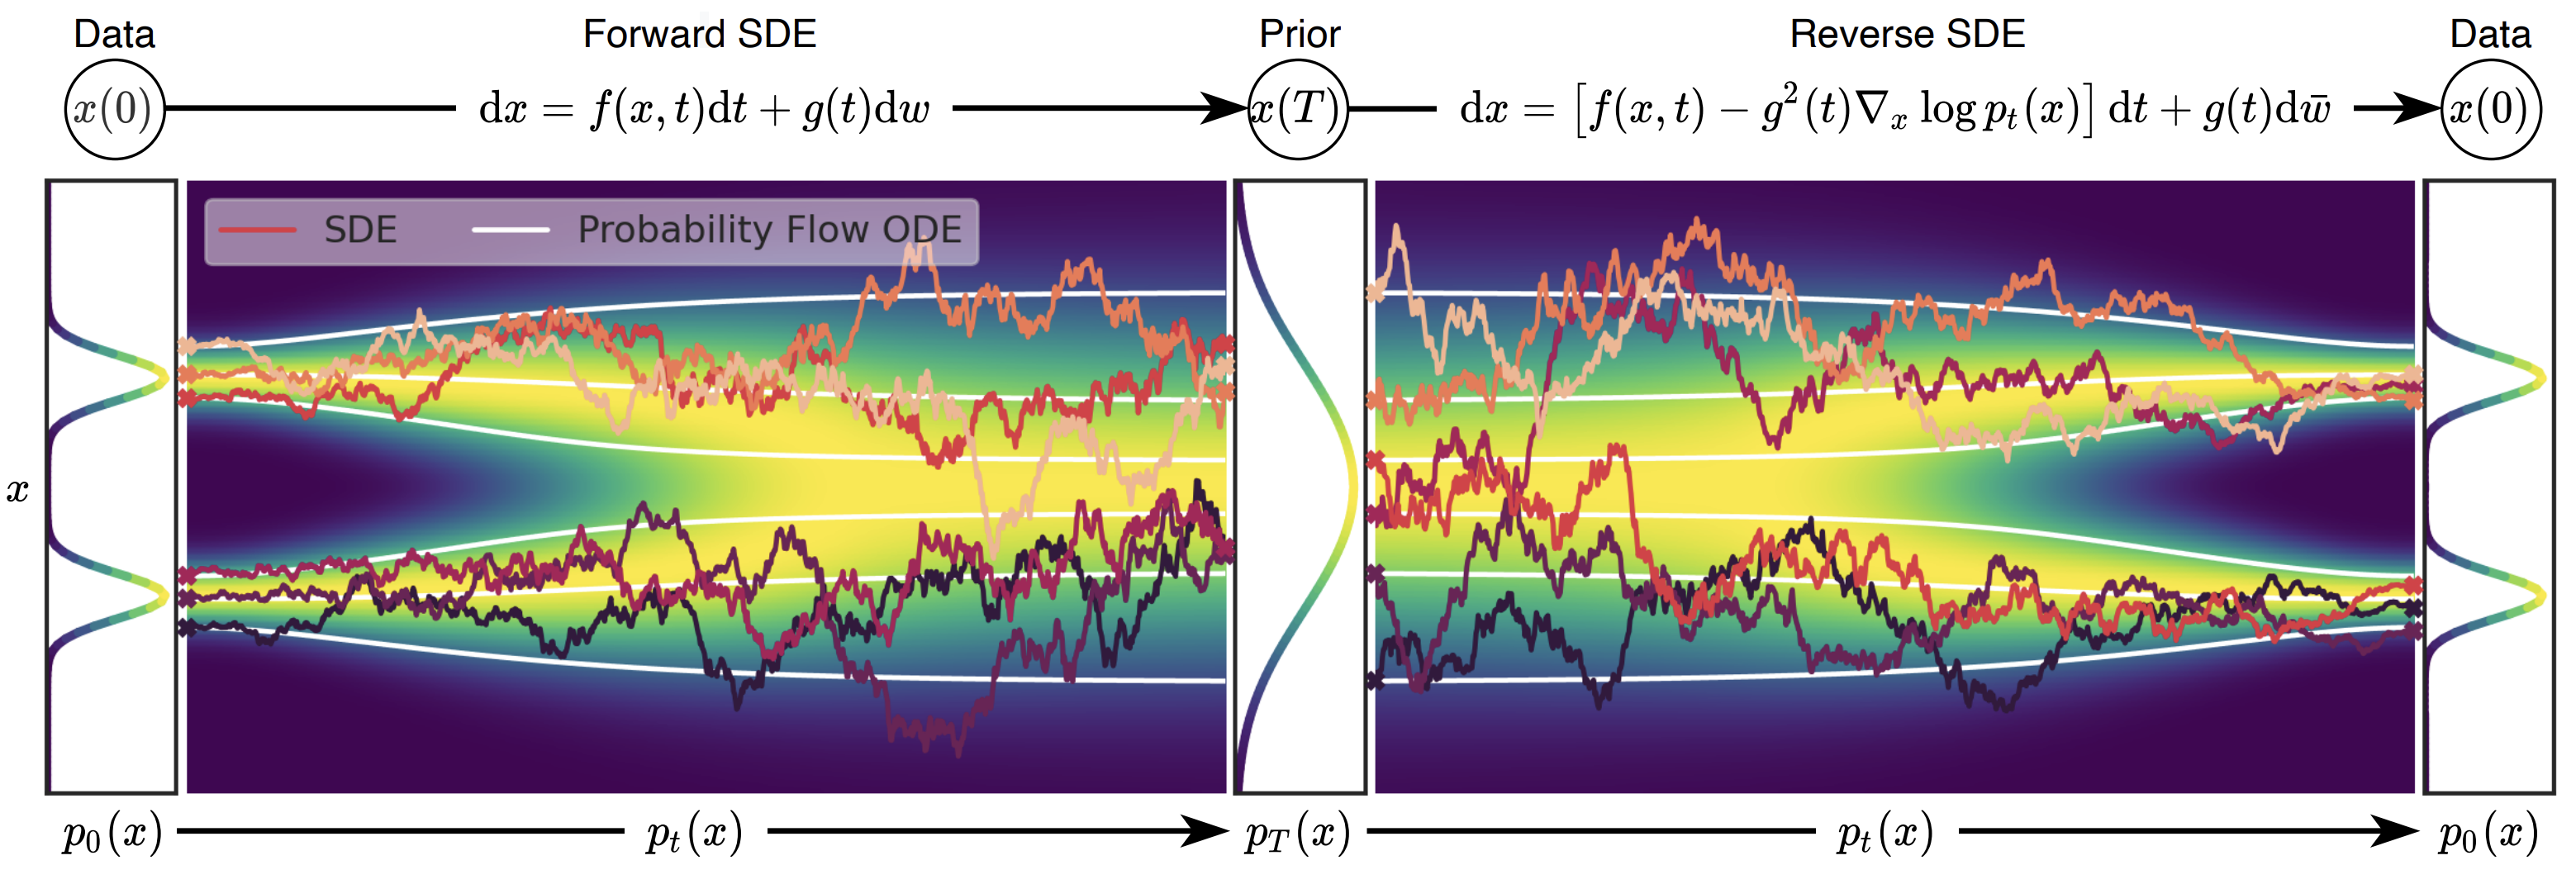
\includegraphics[width=\linewidth]{figs/sde}
	\end{figure}
	\myfootnotewithlink{https://arxiv.org/abs/2011.13456}{Song Y., et al. Score-Based Generative Modeling through Stochastic Differential Equations, 2020}
\end{frame}
%=======
\begin{frame}{Recap of previous lecture}
	\vspace{-0.3cm}
	\[
		d\bx = \mathbf{f}(\bx, t) dt + g(t) d \bw
	\]
	\vspace{-0.3cm}
	\begin{block}{Variance Exploding SDE (NCSN)}
		\vspace{-0.5cm}
		\[
			d \bx = \sqrt{\frac{ d [\sigma^2(t)]}{dt}} \cdot d \bw, \quad \bff(\bx, t) = 0, \quad g(t) = \sqrt{\frac{ d [\sigma^2(t)]}{dt}} 
		\]
		Variance grows since $\sigma(t)$ is a monotonically increasing function.
	\end{block}
	\begin{block}{Variance Preserving SDE (DDPM)}
		\vspace{-0.3cm}
		\[
			d \bx = - \frac{1}{2} \beta(t) \bx(t) dt + \sqrt{\beta(t)} \cdot d \bw
		\]
		\[
			\bff(\bx, t) = - \frac{1}{2} \beta(t) \bx(t) , \quad g(t) = \sqrt{\beta(t)} 
		\]
		Variance is preserved if $\bx(0)$ has a unit variance.
	\end{block}
	\myfootnotewithlink{https://arxiv.org/abs/2011.13456}{Song Y., et al. Score-Based Generative Modeling through Stochastic Differential Equations, 2020}
\end{frame}
%=======
\begin{frame}{Outline}
	\tableofcontents
\end{frame}
%=======
\section{Score-based generative models through SDEs}
%=======
\begin{frame}{Score-based generative models through SDEs}
	\begin{block}{Discrete-in-time objective}
		\vspace{-0.3cm}
		\[
			\bbE_{\pi(\bx_0)} \bbE_{t \sim U\{1, T\}} \bbE_{q(\bx_t | \bx_0)}\bigl\| \bs_{\btheta, t}(\bx_t) - \nabla_{\bx_t} \log q(\bx_t | \bx_0) \bigr\|^2_2 
		\]
		\vspace{-0.3cm}
	\end{block}
	\begin{block}{Continuous-in-time objective}
		\vspace{-0.5cm}
		\[
			\bbE_{\pi(\bx(0))} \bbE_{t \sim U[0, 1]} \bbE_{q(\bx(t) | \bx(0))}\bigl\| \bs_{\btheta}(\bx(t), t) - {\color{teal}\nabla_{\bx(t)} \log q(\bx(t) | \bx(0))} \bigr\|^2_2 
		\]
		\vspace{-0.5cm}
	\end{block}
	\begin{figure}
		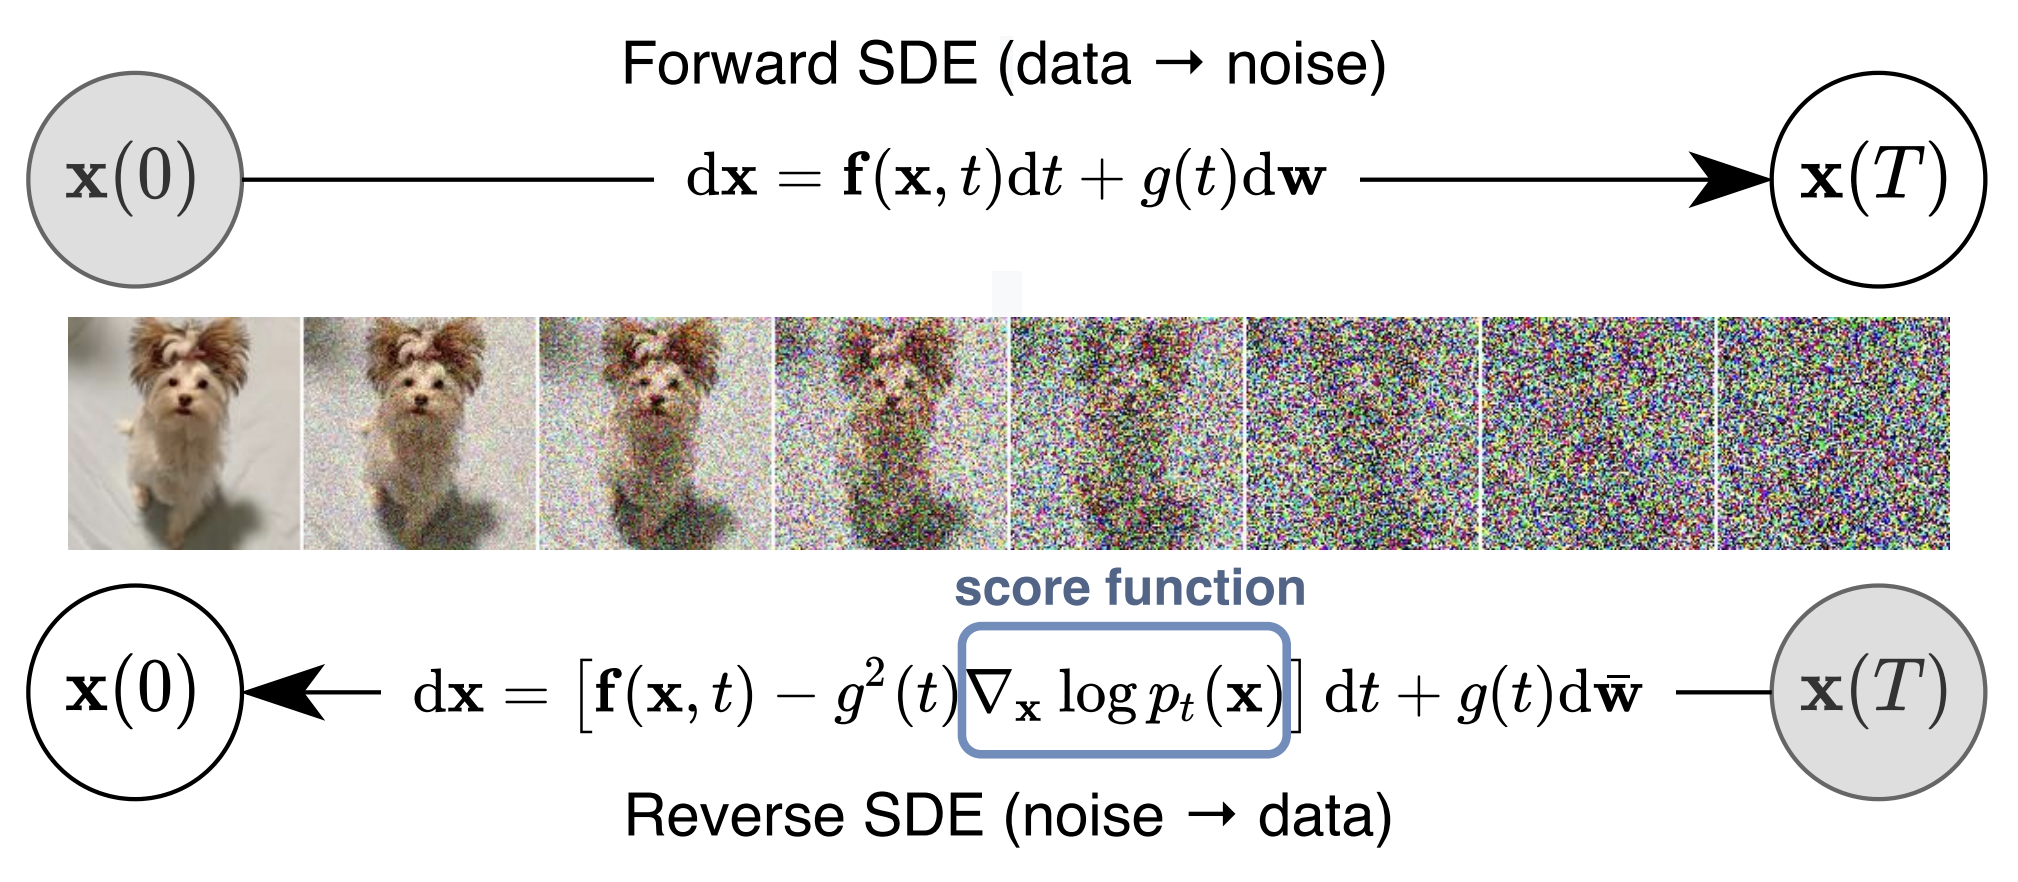
\includegraphics[width=0.8\linewidth]{figs/sbgm}
	\end{figure}
	\myfootnotewithlink{https://arxiv.org/abs/2011.13456}{Song Y., et al. Score-Based Generative Modeling through Stochastic Differential Equations, 2020}
\end{frame}
%=======
\begin{frame}{Score-based generative models through SDEs}
	\vspace{-0.3cm}
	\begin{block}{Continuous-in-time objective}
		\vspace{-0.5cm}
		\[
			\bbE_{\pi(\bx(0))} \bbE_{t \sim U[0, 1]} \bbE_{q(\bx(t) | \bx(0))}\bigl\| \bs_{\btheta}(\bx(t), t) - {\color{teal}\nabla_{\bx(t)} \log q(\bx(t) | \bx(0))} \bigr\|^2_2 
		\]
		\vspace{-0.7cm}
	\end{block}
	\[
		q(\bx(t) | \bx(0)) = \cN\Bigl(\bmu(\bx(t), \bx(0)), \bSigma(\bx(t), \bx(0))\Bigr)
	\]
	\vspace{-0.5cm}
	\begin{block}{Theorem}
		Moments of the SDE $d\bx = \mathbf{f}(\bx, t) dt + g(t) d \bw$ satisfies the equations
		\[
			\frac{d \bmu(\bx(t), \bx(0))}{dt} = \bbE \left[ \bff(\bx(t), t) | \bx(0)\right]
		\]
		\[
			\frac{d \bSigma(\bx(t), \bx(0))}{dt} = \bbE \left[ \bff \cdot (\bx(t) - \bmu)^T + (\bx(t) - \bmu) \cdot \bff^T | \bx(0)\right] + g^2(t) \cdot \bI
		\]
	\end{block}
	Let prove the first one.
	\myfootnotewithlink{https://users.aalto.fi/~asolin/sde-book/sde-book.pdf}{Särkkä S., Solin A. Applied stochastic differential equations, 2019}
\end{frame}
%=======
\begin{frame}{Score-based generative models through SDEs}
	\begin{block}{Theorem}
		\vspace{-0.3cm}
		\[
			\frac{d \bmu(\bx(t), \bx(0))}{dt} = \bbE \left[ \bff(\bx(t), t) | \bx(0)\right]
		\]
		\vspace{-0.5cm}
	\end{block}
	\begin{block}{Proof}
		\vspace{-0.7cm}
		\begin{align*}
			\bbE\left[{\color{violet}d\bx} | \bx(0) \right] &= \bbE\left[{\color{violet}\mathbf{f}(\bx, t) dt} | \bx(0) \right] + \bbE\left[{\color{violet}g(t) d \bw} | \bx(0) \right] \\
			&= \bbE\left[\mathbf{f}(\bx, t) | \bx(0) \right] dt + g(t) \bbE\left[d \bw | \bx(0) \right] \\
			&= \bbE\left[\mathbf{f}(\bx, t) | \bx(0) \right] dt
		\end{align*}
		\[
			\frac{d \bbE\left[\bx | \bx(0) \right]}{dt} = \frac{d \bmu(\bx(t), \bx(0))}{dt} = \bbE\left[\mathbf{f}(\bx, t) | \bx(0) \right] 
		\]
	\end{block}
	\vspace{-0.3cm}
	\begin{block}{Examples}
		\vspace{-0.5cm}
		\[
			\textbf{NCSN:} \quad	\mathbf{f}(\bx, t) = 0 \quad \Rightarrow \quad \bmu = \bx(0)
		\]
		\[
			\textbf{DDPM:} \quad \mathbf{f}(\bx, t) = - \frac{1}{2} \beta(t) \bx(t) \quad \Rightarrow \quad \bmu = \bx(0) \exp\left(- \frac{1}{2} \int_0^t \beta(s)ds\right)
		\]
	\end{block}
	\myfootnotewithlink{https://users.aalto.fi/~asolin/sde-book/sde-book.pdf}{Särkkä S., Solin A. Applied stochastic differential equations, 2019}
\end{frame}
%=======
\begin{frame}{Score-based generative models through SDEs}
	\begin{block}{Training}
		\vspace{-0.5cm}
		\[
			\bbE_{\pi(\bx(0))} \bbE_{t \sim U[0, 1]} \bbE_{q(\bx(t) | \bx(0))}\bigl\| \bs_{\btheta}(\bx(t), t) - {\color{teal}\nabla_{\bx(t)} \log q(\bx(t) | \bx(0))} \bigr\|^2_2 
		\]
		\vspace{-0.7cm}
	\end{block}
	\[
		q(\bx(t) | \bx(0)) = \cN\Bigl(\bmu(\bx(t), \bx(0)), \bSigma(\bx(t), \bx(0))\Bigr)
	\]
	\vspace{-0.5cm}
	\begin{block}{NCSN}
		\vspace{-0.3cm}
		\[
			q(\bx(t) | \bx(0)) = \cN\left(\bx(0), \left[\sigma^2(t) - \sigma^2(0)\right] \cdot \bI\right)
		\]
		\vspace{-0.5cm}
	\end{block}
	\begin{block}{DDPM}
		\vspace{-0.3cm}
		\[
			q(\bx(t) | \bx(0)) = \cN\left(\bx(0) e^{-\frac{1}{2} \int_0^t\beta(s)ds}, \left(1 - e^{- \int_0^t\beta(s)ds}\right) \cdot \bI\right)
		\]
		\vspace{-0.5cm}
	\end{block}
	
	\myfootnotewithlink{https://arxiv.org/abs/2011.13456}{Song Y., et al. Score-Based Generative Modeling through Stochastic Differential Equations, 2020}
\end{frame}
%=======
\begin{frame}{Score-based generative models through SDEs}
	\begin{block}{Sampling}
		Solve reverse SDE using numerical solvers (ODESolve).
		\begin{figure}
			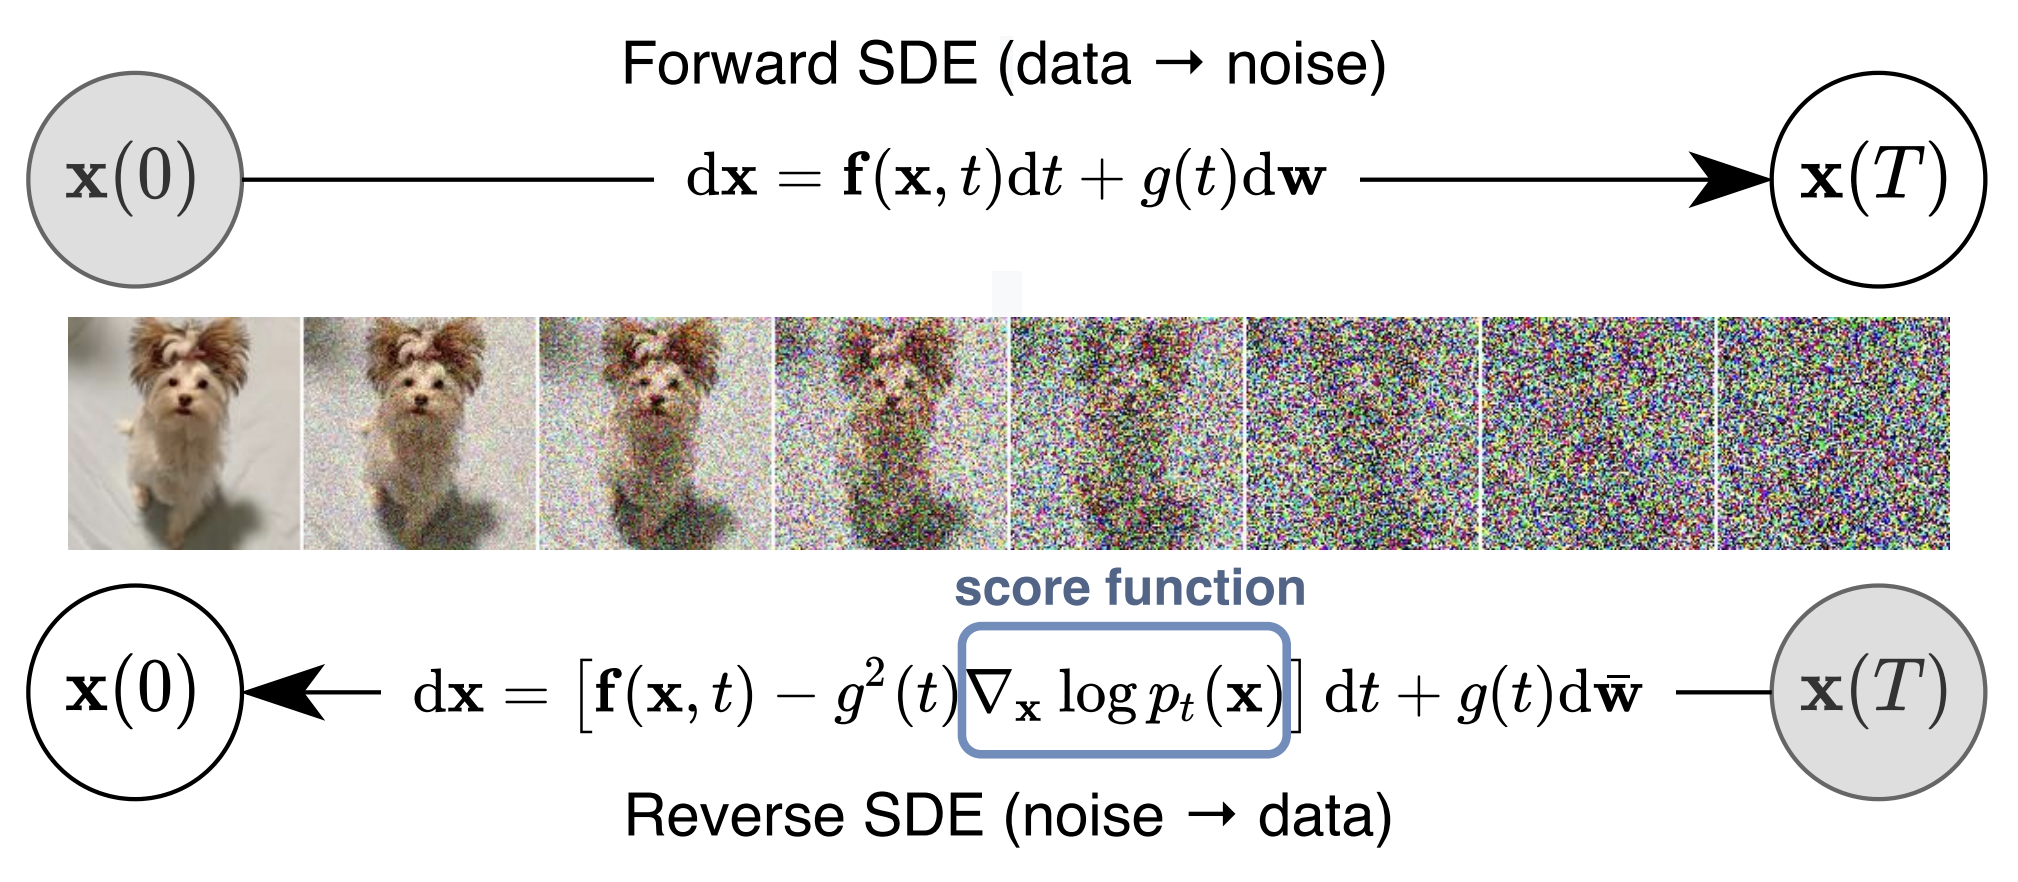
\includegraphics[width=0.8\linewidth]{figs/sbgm}
		\end{figure}
		\vspace{-0.5cm}
	\end{block}
	\begin{itemize}
		\item Discretization of the reverse SDE gives us the ancestral sampling.
		\item If we use probability flow instead of SDE than the reverse ODE gives us the DDIM sampling.
	\end{itemize}
	\myfootnotewithlink{https://arxiv.org/abs/2011.13456}{Song Y., et al. Score-Based Generative Modeling through Stochastic Differential Equations, 2020}
\end{frame}
%=======
\section{Flow Matching}
%=======
\begin{frame}{Continuous-in-time NF}
	Let consider ODE dynamic $\bx(t)$ in time interval $t \in [0, 1]$
	\begin{itemize}
	\item $\bx_0 \sim p_0(\bx) = p(\bx)$, $\bx_1 \sim p_1(\bx) =  \pi(\bx)$;
	\item $p(\bx)$ is a base distribution ($\cN(0, \bI)$) and $\pi(\bx)$ is a true data distribution.
	\end{itemize} 
	\textbf{Note:} the time direction is the same as for CNF (opposite to score-based SDE models).
	\[
		\frac{d \bx}{dt} = \bff (\bx, t),  \quad \text{with initial condition }\bx(0) = \bx_0.
	\]
	\vspace{-0.3cm}
	\begin{block}{KFP theorem (continuity equation)}
		\vspace{-0.5cm}
		\[
			\frac{\partial p_t(\bx)}{\partial t} = - \text{div}\left(\bff(\bx, t) p_t(\bx)\right) \Leftrightarrow \frac{d \log p_t(\bx(t))}{d t} = - \text{tr} \left( \frac{\partial \bff(\bx(t), t)}{\partial \bx(t)} \right)
		\]
		\vspace{-0.3cm}
	\end{block}
	\myfootnotewithlink{https://arxiv.org/abs/1806.07366}{Chen R. T. Q. et al. Neural Ordinary Differential Equations, 2018}   
\end{frame}
%=======
\begin{frame}{Continuous-in-time NF}
	\begin{block}{KFP theorem (continuity equation)}
		\vspace{-0.5cm}
		\[
			\frac{\partial p_t(\bx)}{\partial t} = - \text{div}\left(\bff(\bx, t) p_t(\bx)\right) \Leftrightarrow \frac{d \log p_t(\bx(t))}{d t} = - \text{tr} \left( \frac{\partial \bff(\bx(t), t)}{\partial \bx(t)} \right)
		\]
		\vspace{-0.3cm}
	\end{block}
	\begin{itemize}
		\item If we know the true vector field $\bff (\bx, t)$, then KFP equation (or continuity equation) gives us the way to compute the density $p_t(\bx)$.
		\item Solving the continuity equation using the adjoint method is complicated and unstable process.
		\item \textbf{Flow matching} generalizes these models and gives the alternative way to solve the Neural ODE.
	\end{itemize}
	\begin{block}{Flow Matching}
		\vspace{-0.3cm}
		\[
			\bbE_{t \sim U[0, 1]} \bbE_{\bx \sim p_t(\bx)}\left\| \bff(\bx, t) - \bff_{\btheta}(\bx, t) \right\|^2 \rightarrow \min_{\btheta}
		\]
		\vspace{-0.3cm}
	\end{block}
	\myfootnotewithlink{https://arxiv.org/abs/2210.02747}{Lipman Y., et al. Flow Matching for Generative Modeling, 2022}
\end{frame}
%=======
\begin{frame}{Flow Matching}
	\vspace{-0.3cm}
	\[
		\bbE_{t \sim U[0, 1]} \bbE_{\bx \sim p_t(\bx)}\left\| \bff(\bx, t) - \bff_{\btheta}(\bx, t) \right\|^2 \rightarrow \min_{\btheta}
	\]
	\vspace{-0.3cm}
	\begin{itemize}
		\item There exists infinite number of possible $\bff(\bx, t)$ between $\pi(\bx)$ and $p(\bx)$.
		\item The true vector field  $\bff(\bx, t)$ is \textbf{unknown}.
		\item We need to select the "best" $\bff(\bx, t)$ and makes the objective tractable.
	\end{itemize}
	\begin{figure}
		\centering
		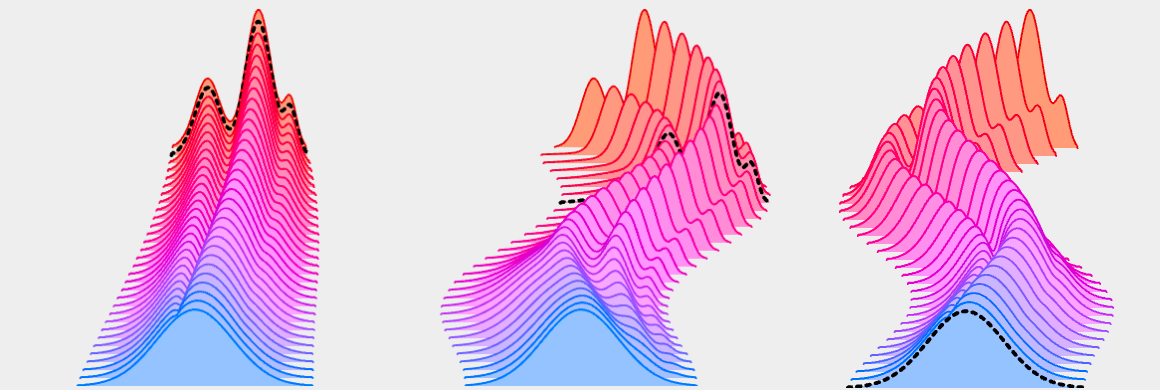
\includegraphics[width=\linewidth]{figs/multiple_dynamics}
	\end{figure}
	\myfootnotewithlink{https://dl.heeere.com/conditional-flow-matching/blog/conditional-flow-matching}{image credit: A Visual Dive into Conditional Flow Matching}
\end{frame}
%=======
\section{Conditional Flow Matching}
%=======
\begin{frame}{Flow Matching}
	\vspace{-0.5cm}
	\begin{block}{Latent variable model}
		Let introduce the latent variable $\bz$:
		\[
			p_t(\bx) = \int p_t(\bx | \bz) p(\bz) d \bz 
		\]
		\vspace{-0.5cm}
	\end{block}
	Here $p_t(\bx | \bz)$ is a \textbf{conditional probability path}.
	
	The conditional probability path $p_t(\bx | \bz)$ satisfies KFP theorem
	\[
		{\color{violet}\frac{\partial p_t(\bx | \bz)}{\partial t} = - \text{div}\left(\bff(\bx, \bz, t) p_t(\bx | \bz)\right)},
	\]
	where $\bff(\bx, \bz, t)$ is a \textbf{conditional vector field}.
	\[
		\frac{d\bx}{dt} = \bff(\bx, t) \quad \Rightarrow \quad \frac{d\bx}{dt} = \bff(\bx, \bz, t)
	\]
	\vspace{-0.3cm}
	What is the relationship between $\bff(\bx, t)$ and $\bff(\bx, \bz, t)$?
	\myfootnotewithlink{https://arxiv.org/abs/2302.00482}{Tong A., et al. Improving and Generalizing Flow-Based Generative Models with Minibatch Optimal Transport, 2023}
\end{frame}
%=======
\begin{frame}{Flow Matching}
	\[
		{\color{violet}\frac{\partial p_t(\bx | \bz)}{\partial t} = - \text{div}\left(\bff(\bx, \bz, t) p_t(\bx | \bz)\right)},
	\]
	\vspace{-0.3cm}
	\begin{block}{Theorem}
		The following vector field generates the probability path $p_t(\bx)$.
		\vspace{-0.2cm}
		\[
			\bff(\bx, t) = \bbE_{p_t(\bz | \bx)} \bff(\bx, \bz, t)  = {\color{teal}\int \bff(\bx, \bz, t)} \frac{\color{teal}p_t(\bx | \bz) p(\bz)}{p_t(\bx)} {\color{teal}d \bz}
		\]
		\vspace{-0.5cm}
	\end{block}
	\begin{block}{Proof}
		\vspace{-0.7cm}
		\begin{multline*}
			\frac{\partial p_t(\bx)}{\partial t} = \frac{\partial}{\partial t} \int p_t(\bx | \bz) p(\bz) d \bz =  \int \left( {\color{violet} \frac{\partial p_t(\bx | \bz)}{\partial t} } \right) p(\bz) d \bz = \\
			= \int \left( {\color{violet} - \text{div}\left(\bff(\bx, \bz, t) p_t(\bx | \bz)\right) } \right) p(\bz) d \bz = \\
			= - \text{div} \left({\color{teal}\int \bff(\bx, \bz, t) p_t(\bx | \bz) p(\bz) d \bz }\right) = - \text{div}  \left(\bff(\bx, t) p_t(\bx)\right)
		\end{multline*}
	\end{block}
	\myfootnotewithlink{https://arxiv.org/abs/2302.00482}{Tong A., et al. Improving and Generalizing Flow-Based Generative Models with Minibatch Optimal Transport, 2023}
\end{frame}
%=======
\begin{frame}{Flow Matching}
	\begin{block}{Flow Matching (FM)}
		\vspace{-0.3cm}
		\[
			\bbE_{t \sim U[0, 1]} \bbE_{\bx \sim p_t(\bx)}\left\| \bff(\bx, t) - \bff_{\btheta}(\bx, t) \right\|^2 \rightarrow \min_{\btheta}
		\]
		\vspace{-0.3cm}
	\end{block}
	\begin{block}{Conditional Flow Matching (CFM)}
		\vspace{-0.3cm}
		\[
			\bbE_{t \sim U[0, 1]} \bbE_{\bz \sim p(\bz)} \bbE_{\bx \sim p_t(\bx | \bz)}\left\| \bff(\bx, \bz, t) - \bff_{\btheta}(\bx, t) \right\|^2 \rightarrow \min_{\btheta}
		\]
		\vspace{-0.3cm}
	\end{block}
	\begin{block}{Theorem}
		If $\text{supp}(p_t(\bx)) = \bbR^m$, then the optimal value of FM objective is equal to the optimal value of CFM objective.
	\end{block}
	\begin{block}{Proof}
		It is proved similarly with the denoising score matching theorem.
	\end{block}
	\myfootnotewithlink{https://arxiv.org/abs/2302.00482}{Tong A., et al. Improving and Generalizing Flow-Based Generative Models with Minibatch Optimal Transport, 2023}
\end{frame}
%=======
\begin{frame}{Conditional Flow Matching}
	\begin{figure}
		\centering
		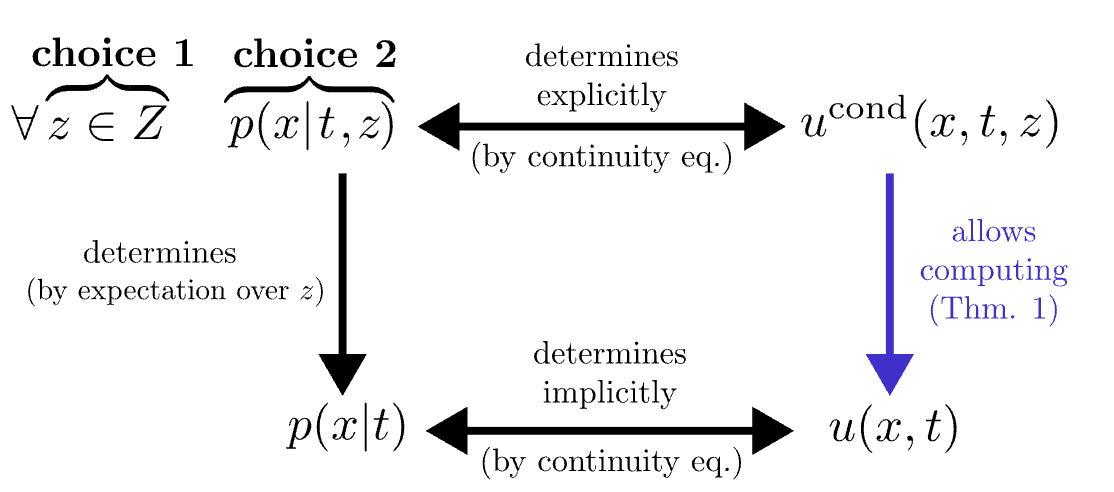
\includegraphics[width=0.75\linewidth]{figs/cfm_uncond_to_cond}
	\end{figure}
	\begin{itemize}
		\item We do not want to model $p_t(\bx)$ because it is complex.
		\item We showed that it is possible to solve CFM task instead of FM task.
		\item Let choose the convenient conditioning latent variable $\bz$.
		\item Let parametrize $p_t(\bx | \bz)$ instead of $p_t(\bx)$. It must satisfy the following constraints
		\[
			p(\bx) = \cN(0, \bI) = \bbE_{p(\bz)} p_0(\bx | \bz); \quad \pi(\bx) = \bbE_{p(\bz)} p_1(\bx | \bz).
		\]
	\end{itemize}
	\myfootnotewithlink{https://dl.heeere.com/conditional-flow-matching/blog/conditional-flow-matching}{image credit: A Visual Dive into Conditional Flow Matching}
\end{frame}
%=======
\begin{frame}{Conditional Flow Matching}
	\vspace{-0.2cm}
	\[
		\bbE_{t \sim U[0, 1]} \bbE_{\bz \sim p(\bz)} \bbE_{\bx \sim p_t(\bx | \bz)}\left\| \bff(\bx, \bz, t) - \bff_{\btheta}(\bx, t) \right\|^2 \rightarrow \min_{\btheta}
	\]
	\vspace{-0.3cm}
	\begin{block}{What is left?}
		\begin{itemize}
			\item How to choose the conditioning latent variable $\bz$?
			\item How to define $p_t(\bx | \bz)$ which follows the constraints?
		\end{itemize}
	\end{block}
	\vspace{-0.3cm}
	\begin{block}{Gaussian conditional probability path}
		\vspace{-0.3cm}
		\[
			p_t(\bx | \bz) = \cN\left(\bmu_t(\bz), \bsigma_t^2(\bz)\right)
		\]
		\vspace{-0.5cm}
	\end{block}
	\begin{itemize}
		\item There is an infinite number of vector fields that generate any particular probability path.
		\item Let consider the following dynamics:
		\[
			\bx_t = \bmu_t(\bz) + \bsigma_t(\bz) \odot \bx_0, \quad {\color{violet} \bx_0 \sim p_0(\bx) = \cN(0, \bI)}
		\]
	\end{itemize}
	\myfootnotewithlink{https://arxiv.org/abs/2302.00482}{Tong A., et al. Improving and Generalizing Flow-Based Generative Models with Minibatch Optimal Transport, 2023}
\end{frame}
%=======
\begin{frame}{Flow Matching}
	\begin{block}{Gaussian conditional probability path}
		\vspace{-0.3cm}
		\[
			p_t(\bx | \bz) = \cN\left(\bmu_t(\bz), \bsigma_t^2(\bz)\right); \quad \bx_t = \bmu_t(\bz) + \bsigma_t(\bz) \odot \bx_0
		\]
		\vspace{-0.5cm}
	\end{block}
	\begin{block}{Theorem}
		\vspace{-0.3cm}
		\[
			\bff(\bx, \bz, t) =  \bmu_t'(\bz) + \frac{\bsigma_t'(\bz)}{\bsigma_t(\bz)} \odot (\bx - \bmu_t(\bz))
		\]
		\vspace{-0.3cm}
	\end{block}
	\begin{block}{Proof}
	\vspace{-0.3cm}
	\[
		\frac{d\bx}{dt} = \bff(\bx, \bz, t); \quad \bx_0 = \frac{1}{\bsigma_t(\bz)} \odot (\bx_t - \bmu_t(\bz))
	\]
	\[
		\frac{d\bx}{dt} = \bmu_t'(\bz) + \bsigma_t'(\bz) \odot \bx_0 =  \bmu_t'(\bz) + \frac{\bsigma_t'(\bz)}{\bsigma_t(\bz)} \odot (\bx - \bmu_t(\bz))
	\]
	\end{block}
	\myfootnotewithlink{https://arxiv.org/abs/2302.00482}{Tong A., et al. Improving and Generalizing Flow-Based Generative Models with Minibatch Optimal Transport, 2023}
\end{frame}
%=======
\subsection{Conical gaussian paths}
%=======
\begin{frame}{Endpoint conditioning}
	\begin{block}{Conditional Flow Matching}
		\vspace{-0.3cm}
		\[
			\bbE_{t \sim U[0, 1]} \bbE_{\bz \sim p(\bz)} \bbE_{\bx \sim p_t(\bx | \bz)}\left\| \bff(\bx, \bz, t) - \bff_{\btheta}(\bx, t) \right\|^2 \rightarrow \min_{\btheta}
		\]
		\vspace{-0.3cm}
	\end{block}
	\begin{block}{Conditioning latent variable}
		Let choose $\bz = \bx_1$. Then $p(\bz) = p_1(\bx_1)$.
		\[
			p_t(\bx) = \int p_t(\bx | \bx_1) p_1(\bx_1) d \bx_1
		\]
	\end{block}
	We need to ensure boundary constraints:
	\[
		\begin{cases}
			p(\bx) = \bbE_{p(\bz)} p_0(\bx | \bz); {\color{gray}(= \cN(0, \bI))} \\
			\pi(\bx) = \bbE_{p(\bz)} p_1(\bx | \bz).
		\end{cases}
		\quad \Rightarrow \quad 
		\begin{cases}
			p_0(\bx | \bx_1) = \cN(0, \bI); \\
			p_1(\bx | \bx_1) = \delta(\bx - \bx_1).
		\end{cases}
	\]
	\vspace{-0.3cm}
	\myfootnotewithlink{https://arxiv.org/abs/2210.02747}{Lipman Y., et al. Flow Matching for Generative Modeling, 2022}
\end{frame}
%=======
\begin{frame}{Conical gaussian paths}
	\[
		p_0(\bx | \bx_1) = \cN(0, \bI); \quad p_1(\bx | \bx_1) = \delta(\bx - \bx_1).
	\]
	
	\begin{block}{Gaussian conditional probability path}
		\vspace{-0.5cm}
		\[
			p_t(\bx | \bx_1) = \cN\left(\bmu_t(\bx_1), \bsigma_t^2(\bx_1)\right); \quad \bx_t = \bmu_t(\bx_1) +  \bsigma_t^2(\bx_1) \odot \bx_0.
		\]
		\vspace{-0.6cm}
	\end{block}
	Let consider straight conditional paths	
	\[
		\begin{cases}
			\bmu_t(\bx_1) = t \bx_1; \\
			\bsigma_t(\bx_1) = (1 - t).
		\end{cases}
		\quad \Rightarrow \quad 
		\begin{cases}
			p_t(\bx | \bx_1) = \cN\left(t \bx_1, (1-t)^2 \bI\right); \\
		 	\bx_t = t \bx_1 + (1 - t) \bx_0. 
	 \end{cases}
	\]
	\vspace{-0.3cm}
	\begin{figure}
		\centering
		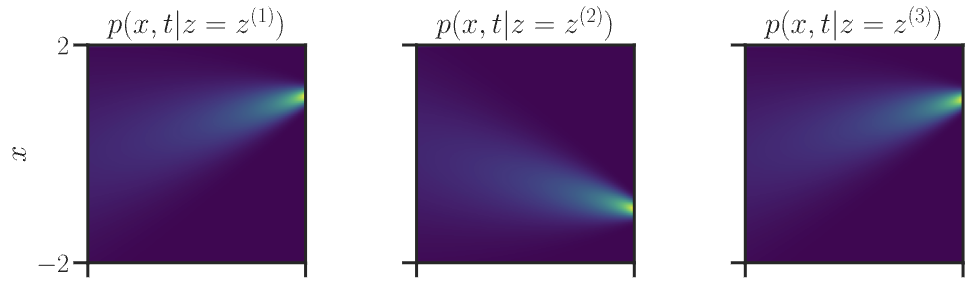
\includegraphics[width=\linewidth]{figs/conical_paths}
	\end{figure}
	\myfootnotewithlink{https://dl.heeere.com/conditional-flow-matching/blog/conditional-flow-matching}{image credit: A Visual Dive into Conditional Flow Matching}
\end{frame}
%=======
\begin{frame}{Conical gaussian paths}
	\vspace{-0.3cm}
	\[
		p_t(\bx | \bx_1) = \cN\left(t \bx_1, (1-t)^2 \bI\right); \quad {\color{teal}\bx_t = t \bx_1 + (1 - t) \bx_0}. 
	\]
	\vspace{-0.5cm}
	\begin{block}{Conditional vector field}
		\vspace{-0.3cm}
		\[
			 \frac{d\bx}{dt} = \bff(\bx, \bx_1, t) =  \bmu_t'(\bx_1) + \frac{\bsigma_t'(\bx_1)}{\bsigma_t(\bx_1)} \odot (\bx - \bmu_t(\bx_1))
		\]
		\vspace{-0.5cm}
		\begin{multline*}
			\bff(\bx, \bx_1, t) = \bx_1 - \frac{1}{1-t} \cdot (\bx - t \bx_1) = \frac{\bx_1 - {\color{teal}\bx}}{1-t} = \\
			= \frac{\bx_1 - {\color{teal}t \bx_1 + (1 - t) \bx_0}}{1-t} = \bx_1 - \bx_0
		\end{multline*}
		\vspace{-0.7cm}
	\end{block}
	\begin{block}{Conditional Flow Matching}
		\vspace{-0.7cm}
		\begin{multline*}
			\bbE_{t \sim U[0, 1]} \bbE_{\bz \sim p(\bz)} \bbE_{\bx \sim p_t(\bx | \bz)}\left\| \bff(\bx, \bz, t) - \bff_{\btheta}(\bx, t) \right\|^2 = \\
		 \bbE_{t \sim U[0, 1]} \bbE_{\bx_1 \sim \pi(\bx)} \bbE_{\bx \sim p_t(\bx | \bx_1)}\left\| \left(\frac{\bx_1 - \bx}{1-t}\right) - \bff_{\btheta}(\bx, t) \right\|^2 = \\
		 \bbE_{t \sim U[0, 1]} \bbE_{\bx_1 \sim \pi(\bx)} \bbE_{\bx_0 \sim \cN(0, \bI)}\left\| (\bx_1 - \bx_0) - \bff_{\btheta}\left(t \bx_1 + (1 - t) \bx_0, t\right) \right\|^2
		\end{multline*}
		\vspace{-0.5cm}
	\end{block}	
	\myfootnotewithlink{https://arxiv.org/abs/2210.02747}{Lipman Y., et al. Flow Matching for Generative Modeling, 2022}
\end{frame}
%=======
\begin{frame}{Conditional Flow Matching}
	\vspace{-0.3cm}
	\[
	 \bbE_{t \sim U[0, 1]} \bbE_{\bx_1 \sim \pi(\bx)} \bbE_{\bx_0 \sim \cN(0, \bI)}\left\| (\bx_1 - \bx_0) - \bff_{\btheta}(\bx, t) \right\|^2  \rightarrow \min_{\btheta}
	\]
	We fit straight lines between noise distribution $p(\bx)$ and the data distribution $\pi(\bx)$.
	\begin{block}{Training}
		\begin{enumerate}
			\item Get the sample $\bx_1 \sim \pi(\bx)$.
			\item Sample timestamp $t \sim U\{1, T\}$ and $\bx_0 \sim \cN(0, \bI)$.
			\item Get noisy image $\bx_t = \sqrt{\bar{\alpha}_t} \cdot \bx_0 + \sqrt{1 - \bar{\alpha}_t} \cdot \bepsilon$.
			\item Compute loss $ \cL = \left\| (\bx_1 - \bx_0) - \bff_{\btheta}(\bx, t) \right\|^2 $.
		\end{enumerate}
	\end{block}
	\vspace{-0.3cm}
	\begin{block}{Sampling}
		\begin{enumerate}
			\item Sample $\bx_0 \sim \cN(0, \bI)$.
			\item Solve the ODE to get $\bx_1$:
			\[
				\bx_1 = \text{ODESolve}_f(\bx_0, \btheta, t_0=0, t_1=1).
			\]
		\end{enumerate}
	\end{block}
	\myfootnotewithlink{https://arxiv.org/abs/2210.02747}{Lipman Y., et al. Flow Matching for Generative Modeling, 2022}
\end{frame}
%=======
\begin{frame}{Flow Matching}
	\[
		\bx_t = t \bx_1 + (1 - t) \bx_0
	\]
	\vspace{-0.3cm}
	\begin{itemize}
		\item The conditional probability path $p_t(\bx|\bz)$ is an \textbf{optimal transport path} from $p_0(\bx|\bz)$ to $p_1(\bx|\bz)$ (in terms of the conditional trajectories straightness).
		\item The marginal path $p_t(\bx)$ is not in general an optimal transport path from the standard normal $p_0(\bx)$ to the data distribution $p_1(\bx)$.
	\end{itemize}
	\begin{minipage}[t]{0.5\columnwidth}
			\begin{figure}
				\centering
				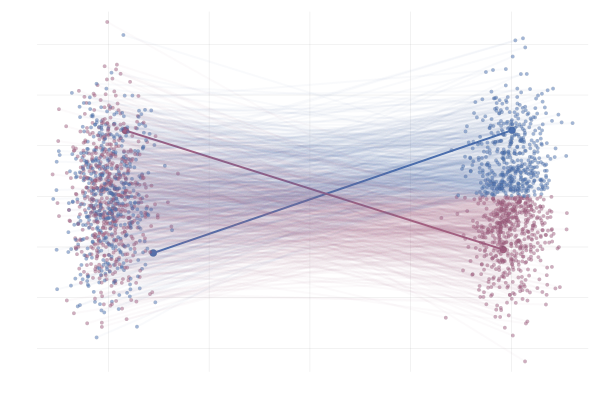
\includegraphics[width=\linewidth]{figs/g2g-vector-field-samples-cond}
			\end{figure}
		\end{minipage}%
		\begin{minipage}[t]{0.5\columnwidth}
			\begin{figure}
				\centering
				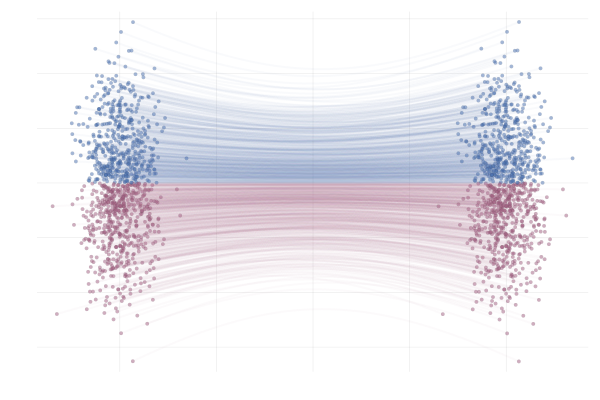
\includegraphics[width=\linewidth]{figs/g2g-forward_samples}
			\end{figure}
	\end{minipage}
	\myfootnotewithlink{https://mlg.eng.cam.ac.uk/blog/2024/01/20/flow-matching.html}{image credit: https://mlg.eng.cam.ac.uk/blog/2024/01/20/flow-matching.html}
\end{frame}
%=======
\subsection{Link with score-based models}
%=======
\begin{frame}{Flow matching vs score-based SDE models}
	\begin{block}{Flow matching probability path}
		\vspace{-0.3cm}
		\[
			p_t(\bx | \bx_1) = \cN\left(t \bx_1, (1-t)^2 \bI\right); \quad \bff(\bx, \bx_1, t) = \frac{\bx_1  - \bx}{1-t}
		\]
		\vspace{-0.3cm}
	\end{block}
	\begin{block}{Variance Exploding SDE probability path}
		\vspace{-0.3cm}
		\[
			d \bx = \sqrt{\frac{ d [\sigma^2(t)]}{dt}} \cdot d \bw;
			\quad \Rightarrow \quad
			\begin{cases}
				p_t(\bx | \bx_1) = \cN\left(\bx_1, \sigma^2_{1-t}  \bI\right) \\
				\bff(\bx, \bx_1, t) = - \frac{\sigma'_{1-t}}{\sigma_{1-t}} \cdot (\bx - \bx_1)
			\end{cases}
		\]
		\vspace{-0.3cm}
	\end{block}
	\begin{block}{Variance Preserving SDE probability path}
		\vspace{-0.3cm}
		{\small
		\[
			d \bx = - \frac{1}{2} \beta(t) \bx(t) dt + \sqrt{\beta(t)} d \bw;
			\, \Rightarrow \,
			\begin{cases}
				p_t(\bx | \bx_1) = \cN\left(\alpha_{1-t}  \bx_1, (1 - \alpha^2_{1-t})  \bI \right) \\
				\bff(\bx, \bx_1, t) = \frac{\alpha'_{1-t}}{1 - \alpha^2_{1-t}}\cdot \left(\alpha_{1-t}  \bx - \bx_1\right)
			\end{cases}
		\]
		}
		Here $\alpha_t = \exp\left({-\frac{1}{2} \int_0^t \beta(s) ds} \right)$.
	\end{block}
	\myfootnotewithlink{https://arxiv.org/abs/2210.02747}{Lipman Y., et al. Flow Matching for Generative Modeling, 2022}
\end{frame}
%=======
\begin{frame}{Flow matching vs score-based SDE models}
	\begin{block}{Diffusion vector field}
		\begin{figure}
			\centering
			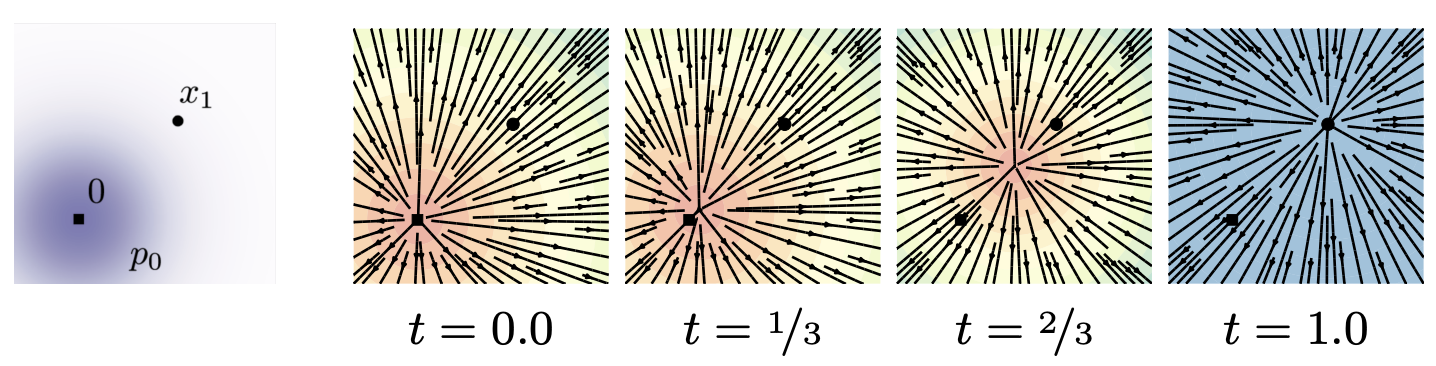
\includegraphics[width=\linewidth]{figs/diff_cond_path}
		\end{figure}
	\end{block}
	\begin{block}{Flow matching vector field}
		\begin{figure}
			\raggedleft
			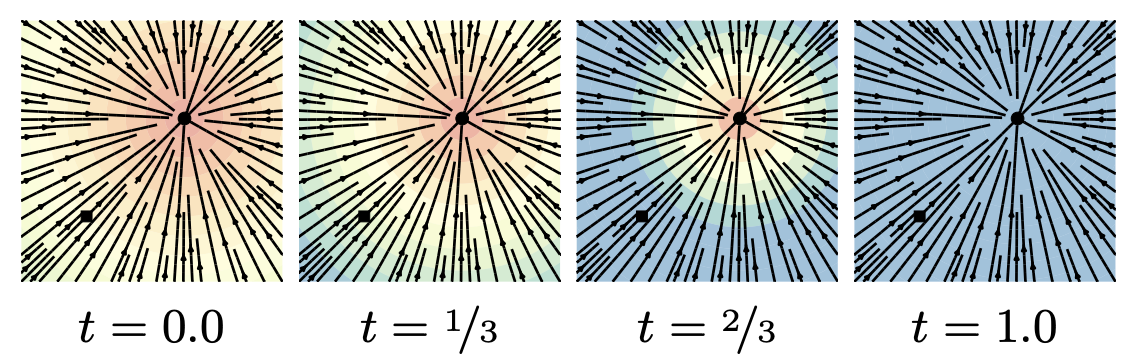
\includegraphics[width=0.77\linewidth]{figs/ot_cond_path}
		\end{figure}
	\end{block}
	\myfootnotewithlink{https://arxiv.org/abs/2210.02747}{Lipman Y., et al. Flow Matching for Generative Modeling, 2022}
\end{frame}
%=======
\begin{frame}{Flow matching vs score-based SDE models}
	\begin{figure}
		\centering
		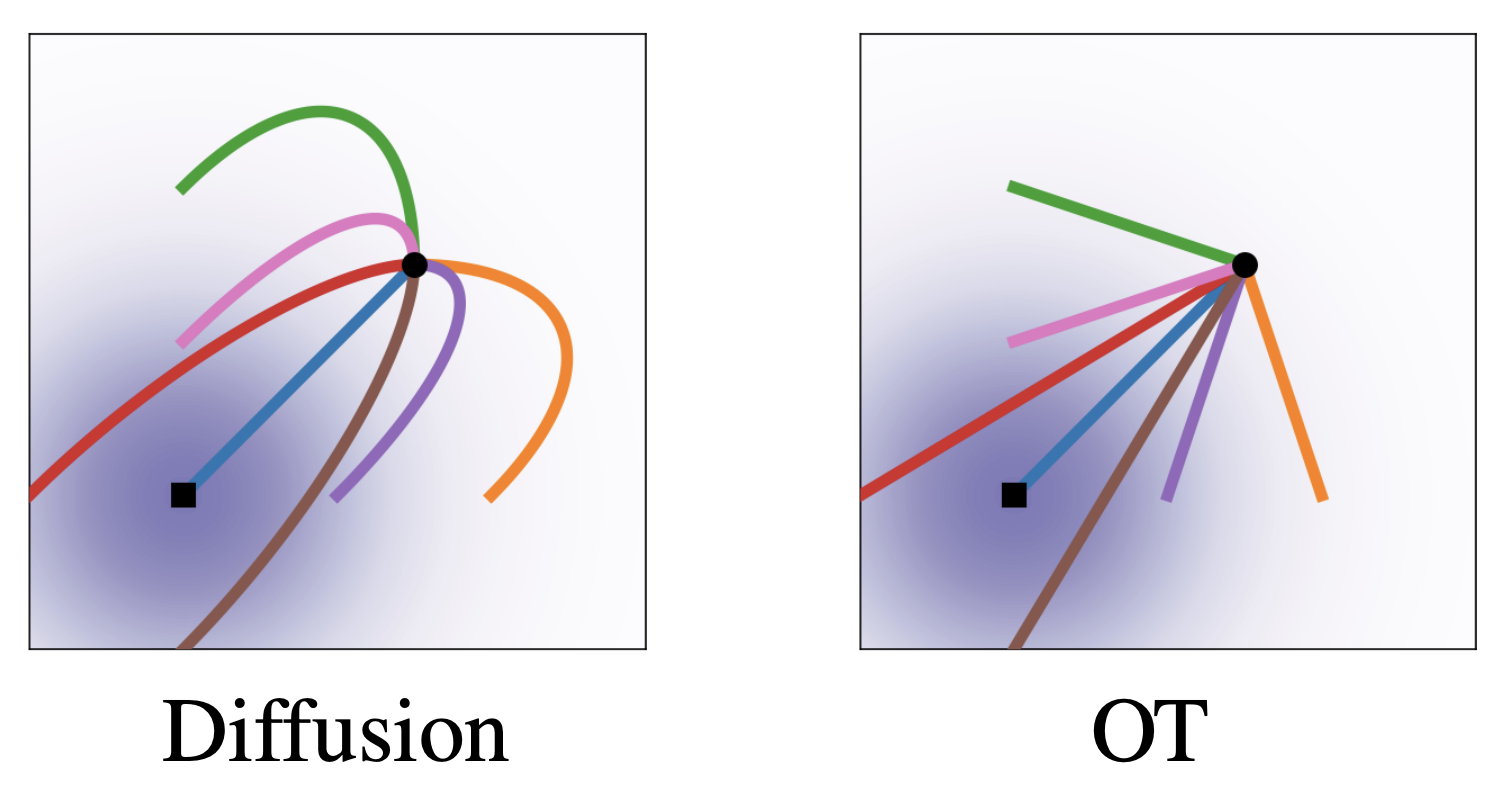
\includegraphics[width=0.7\linewidth]{figs/trajectories}
	\end{figure}
	\begin{figure}
		\centering
		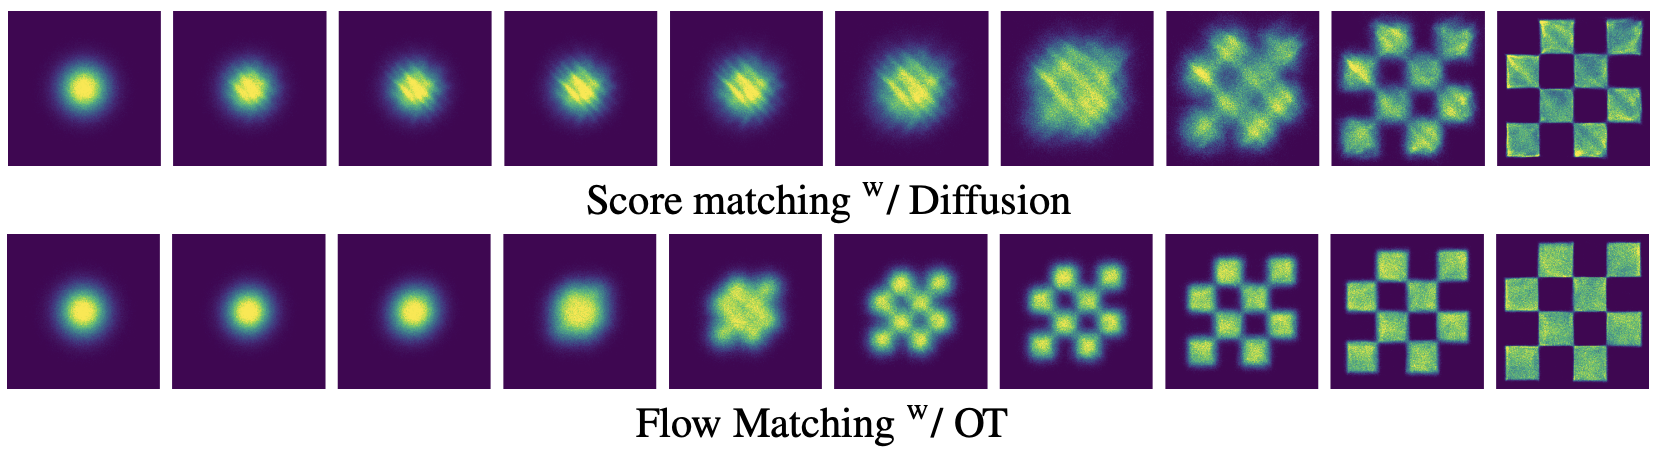
\includegraphics[width=\linewidth]{figs/2d-generation}
	\end{figure}
	\myfootnotewithlink{https://arxiv.org/abs/2210.02747}{Lipman Y., et al. Flow Matching for Generative Modeling, 2022}
\end{frame}
%=======
\begin{frame}{Summary}
	\begin{itemize}
		\item It is possible to train the continuous-in-time score-based generative models through forward and reverse SDEs.
		\vfill
		\item Discretization of the reverse SDE gives the ancestral sampling of the DDPM.
		\vfill
		\item Flow matching suggests to fit the vector field directly.
		\vfill
		\item Conditional flow matching allows to make the FM objective tractable.
		\vfill
		\item Conical gaussian paths is the example of the effective FM technique.
	\end{itemize}
\end{frame}
\end{document} 